\section{Experimental Results}

To compare the cache performance of Van Emde-Boas trees and binary search trees, we conducted a series of experiments. We measured the number of cache misses for various sizes of the universe (B) and recorded the results.

\subsection{Setup}

The experiments were conducted on a machine with the following specifications:
\begin{itemize}
    \item Processor: M2 Mac (Apple Silicon)
    \item RAM: 16GB
    \item Cache: 16 KB 4-way set associative L1 instruction and data caches, 256 KB 8-way set associative L2 cache, all with 64-byte lines. (informations from \code{valgrind ... -v ...})
\end{itemize}

\subsection{Experimental Procedure}
\begin{enumerate}
    \item We implemented Van Emde-Boas trees and binary search trees in Python.
    \item We used Valgrind's Cachegrind tool to measure the number of cache misses for each data structure.
    \item We varied the size of the universe (B) and recorded the number of cache misses for each configuration.
        \begin{multicols}{2}
        \begin{itemize}
            \item 256
            \item 512
            \item 1024
            \item 2048
            \item 4096
            \item 8192
            \item 16384
        \end{itemize}
    \end{multicols}
    \item We repeated the experiments multiple times to ensure the consistency of the results.
    \item We analyzed the results to compare the cache performance of Van Emde-Boas trees and binary search trees.
    \item We generated tables and figures to summarize the results.
    \item We interpreted the results to draw conclusions about the cache performance of the two data structures.
\end{enumerate}

\subsection{Results}
The following tables and figures summarize the cache misses for different configurations of B.
\begin{table}[h!]
    \centering
    {\small
    \begin{tabular}{lrrrrrrrr}
        \toprule
        & & 256 & 512 & 1024 & 2048 & 4096 & 8192 & 16384 \\
        \midrule
        \multirow{5}{*}{VEB}
        & Instruction cache misses & 586,338 & 656,874 & 747,164 & 944,139 & 1,298,782 & 1,923,825 & 3,138,048 \\
        & Data cache read misses & 826,978 & 914,641 & 1,093,725 & 1,323,708 & 1,782,222 & 2,581,843 & 4,114,636 \\
        & Last-level cache read misses & 342,641 & 362,002 & 465,148 & 563,046 & 784,288 & 1,136,228 & 1,839,706 \\
        & Data cache write misses & 86,317 & 95,840 & 105,986 & 127,986 & 167,471 & 239,100 & 355,242 \\
        & Last-level cache write misses & 48,242 & 50,590 & 53,554 & 60,146 & 71,901 & 91,876 & 130,123 \\
        \midrule
        \multirow{5}{*}{BST}
        & Instruction cache misses & 486,541 & 493,182 & 503,951 & 525,072 & 565,804 & 648,061 & 812,394 \\
        & Data cache read misses & 786,192 & 806,564 & 850,909 & 967,983 & 1,280,734 & 1,769,552 & 2,897,689 \\
        & Last-level cache read misses & 333,316 & 336,076 & 340,758 & 352,443 & 463,768 & 614,714 & 1,007,555 \\
        & Data cache write misses & 72,848 & 74,668 & 78,745 & 88,967 & 110,487 & 145,009 & 241,735 \\
        & Last-level cache write misses & 40,881 & 41,268 & 42,107 & 43,857 & 47,511 & 55,565 & 72,183 \\
        \bottomrule
    \end{tabular}
    }
    \caption{Cache misses for VEB and BST}
\end{table}

\begin{figure}[h!]
    \centering
    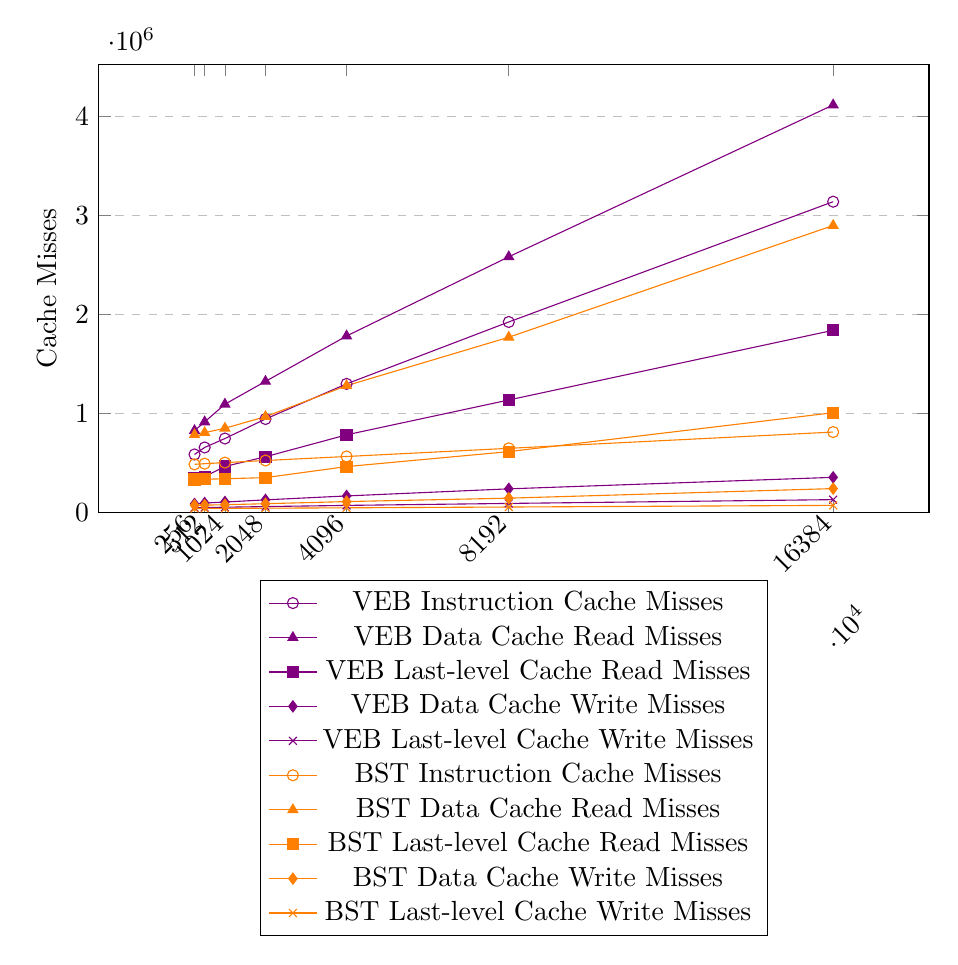
\begin{tikzpicture}
        \begin{axis}[
            width=\textwidth,
            height=0.6\textwidth,
            xlabel={Block Size},
            ylabel={Cache Misses},
            xtick={256, 512, 1024, 2048, 4096, 8192, 16384},
            xticklabels={256, 512, 1024, 2048, 4096, 8192, 16384},
            ymin=0,
            ymajorgrids=true,
            grid style=dashed,
            cycle list name=color list,
            enlarge x limits=0.15,
            xticklabel style={rotate=45, anchor=east},
            legend style={at={(0.5,-0.15)},anchor=north}
        ]
        \addplot+[mark=o, color=violet] table[x index=0, y index=1, col sep=comma] {
            BlockSize,InstructionCacheMisses
            256,586338
            512,656874
            1024,747164
            2048,944139
            4096,1298782
            8192,1923825
            16384,3138048
        };
        \addplot+[mark=triangle*, color=violet] table[x index=0, y index=1, col sep=comma] {
            BlockSize,DataCacheReadMisses
            256,826978
            512,914641
            1024,1093725
            2048,1323708
            4096,1782222
            8192,2581843
            16384,4114636
        };
        \addplot+[mark=square*, color=violet] table[x index=0, y index=1, col sep=comma] {
            BlockSize,LastLevelCacheReadMisses
            256,342641
            512,362002
            1024,465148
            2048,563046
            4096,784288
            8192,1136228
            16384,1839706
        };
        \addplot+[mark=diamond*, color=violet] table[x index=0, y index=1, col sep=comma] {
            BlockSize,DataCacheWriteMisses
            256,86317
            512,95840
            1024,105986
            2048,127986
            4096,167471
            8192,239100
            16384,355242
        };
        \addplot+[mark=x, color=violet] table[x index=0, y index=1, col sep=comma] {
            BlockSize,LastLevelCacheWriteMisses
            256,48242
            512,50590
            1024,53554
            2048,60146
            4096,71901
            8192,91876
            16384,130123
        };
        \addplot+[mark=o, color=orange] table[x index=0, y index=1, col sep=comma] {
            BlockSize,InstructionCacheMisses
            256,486541
            512,493182
            1024,503951
            2048,525072
            4096,565804
            8192,648061
            16384,812394
        };
        \addplot+[mark=triangle*, color=orange] table[x index=0, y index=1, col sep=comma] {
            BlockSize,DataCacheReadMisses
            256,786192
            512,806564
            1024,850909
            2048,967983
            4096,1280734
            8192,1769552
            16384,2897689
        };
        \addplot+[mark=square*, color=orange] table[x index=0, y index=1, col sep=comma] {
            BlockSize,LastLevelCacheReadMisses
            256,333316
            512,336076
            1024,340758
            2048,352443
            4096,463768
            8192,614714
            16384,1007555
        };
        \addplot+[mark=diamond*, color=orange] table[x index=0, y index=1, col sep=comma] {
            BlockSize,DataCacheWriteMisses
            256,72848
            512,74668
            1024,78745
            2048,88967
            4096,110487
            8192,145009
            16384,241735
        };
        \addplot+[mark=x, color=orange] table[x index=0, y index=1, col sep=comma] {
            BlockSize,LastLevelCacheWriteMisses
            256,40881
            512,41268
            1024,42107
            2048,43857
            4096,47511
            8192,55565
            16384,72183
        };
        \legend{VEB Instruction Cache Misses,
                VEB Data Cache Read Misses,
                VEB Last-level Cache Read Misses,
                VEB Data Cache Write Misses,
                VEB Last-level Cache Write Misses,
                BST Instruction Cache Misses,
                BST Data Cache Read Misses,
                BST Last-level Cache Read Misses,
                BST Data Cache Write Misses,
                BST Last-level Cache Write Misses}
        \end{axis}
    \end{tikzpicture}
    \caption{Cache misses for VEB and BST}
    \label{fig:cache_misses}
\end{figure}

\subsection{Time Analysis}
The following plot shows the time taken for insert and search operations for Van Emde-Boas trees and binary search trees. The full code for generating this plot is provided in the appendix \ref{appendix:time_performance_plot}.
\begin{figure}[h]
\centering
    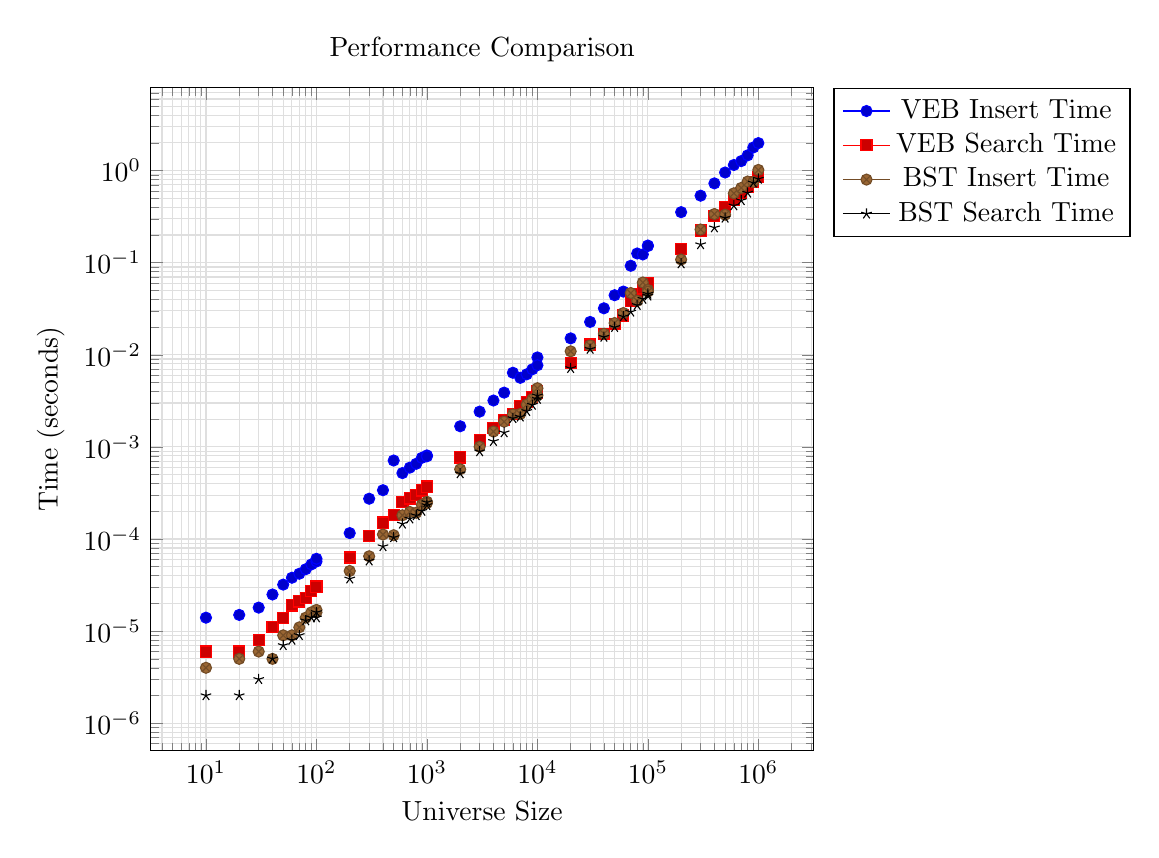
\begin{tikzpicture}
        \begin{axis}[
            title={Performance Comparison},
            xlabel={Universe Size},
            ylabel={Time (seconds)},
            xmode=log,
            ymode=log,
            legend pos=outer north east,
            grid=both,
            minor grid style={gray!25},
            major grid style={gray!25},
            width=10cm,
            height=10cm,
        ]

        \addplot coordinates {
        
            (10, 1.4000000000000123e-05)
        
            (20, 1.4999999999994185e-05)
        
            (30, 1.8000000000004124e-05)
        
            (40, 2.4999999999997247e-05)
        
            (50, 3.199999999999731e-05)
        
            (60, 3.800000000000331e-05)
        
            (70, 4.200000000000037e-05)
        
            (80, 4.700000000000537e-05)
        
            (90, 5.300000000000443e-05)
        
            (100, 5.7000000000001494e-05)
        
            (100, 6.0999999999998555e-05)
        
            (200, 0.00011600000000000499)
        
            (300, 0.00027399999999999647)
        
            (400, 0.000338999999999999)
        
            (500, 0.0007119999999999974)
        
            (600, 0.0005199999999999996)
        
            (700, 0.0005959999999999924)
        
            (800, 0.0006560000000000038)
        
            (900, 0.0007619999999999988)
        
            (1000, 0.0008089999999999903)
        
            (1000, 0.000791)
        
            (2000, 0.001676999999999998)
        
            (3000, 0.0024180000000000035)
        
            (4000, 0.0031909999999999994)
        
            (5000, 0.0038880000000000026)
        
            (6000, 0.006389000000000006)
        
            (7000, 0.005627999999999994)
        
            (8000, 0.006143999999999983)
        
            (9000, 0.006963999999999998)
        
            (10000, 0.009372999999999992)
        
            (10000, 0.00770800000000002)
        
            (20000, 0.015093999999999996)
        
            (30000, 0.02276600000000001)
        
            (40000, 0.032016000000000044)
        
            (50000, 0.04438800000000004)
        
            (60000, 0.04861599999999999)
        
            (70000, 0.09270800000000001)
        
            (80000, 0.12599899999999997)
        
            (90000, 0.12299899999999986)
        
            (100000, 0.15362199999999993)
        
            (100000, 0.15198299999999998)
        
            (200000, 0.3541810000000001)
        
            (300000, 0.5345530000000003)
        
            (400000, 0.7273519999999998)
        
            (500000, 0.9544100000000002)
        
            (600000, 1.151159999999999)
        
            (700000, 1.2694739999999989)
        
            (800000, 1.466095000000001)
        
            (900000, 1.784718999999999)
        
            (1000000, 1.9902820000000006)
        
        };
        \addlegendentry{VEB Insert Time}

        \addplot coordinates {
        
            (10, 5.999999999999062e-06)
        
            (20, 6.0000000000060005e-06)
        
            (30, 7.999999999994123e-06)
        
            (40, 1.1000000000004062e-05)
        
            (50, 1.4000000000000123e-05)
        
            (60, 1.8999999999998185e-05)
        
            (70, 2.1000000000000185e-05)
        
            (80, 2.2999999999995246e-05)
        
            (90, 2.6999999999999247e-05)
        
            (100, 3.099999999999631e-05)
        
            (100, 3.0000000000002247e-05)
        
            (200, 6.300000000000056e-05)
        
            (300, 0.00010800000000000393)
        
            (400, 0.00015099999999999836)
        
            (500, 0.00018399999999999667)
        
            (600, 0.0002530000000000032)
        
            (700, 0.00027599999999999847)
        
            (800, 0.0003010000000000096)
        
            (900, 0.0003369999999999901)
        
            (1000, 0.00038000000000000533)
        
            (1000, 0.0003700000000000092)
        
            (2000, 0.0007690000000000058)
        
            (3000, 0.0011820000000000025)
        
            (4000, 0.0016019999999999923)
        
            (5000, 0.0019639999999999935)
        
            (6000, 0.0022979999999999945)
        
            (7000, 0.0027810000000000057)
        
            (8000, 0.0030930000000000124)
        
            (9000, 0.003485999999999989)
        
            (10000, 0.0038930000000000076)
        
            (10000, 0.0040869999999999795)
        
            (20000, 0.008152999999999994)
        
            (30000, 0.012925999999999993)
        
            (40000, 0.016742999999999952)
        
            (50000, 0.02147199999999999)
        
            (60000, 0.026714999999999933)
        
            (70000, 0.038515999999999995)
        
            (80000, 0.0455890000000001)
        
            (90000, 0.05261999999999989)
        
            (100000, 0.06001699999999999)
        
            (100000, 0.06068499999999988)
        
            (200000, 0.14119400000000004)
        
            (300000, 0.22347599999999979)
        
            (400000, 0.3185880000000001)
        
            (500000, 0.4023570000000003)
        
            (600000, 0.48375900000000094)
        
            (700000, 0.5740680000000005)
        
            (800000, 0.6603290000000008)
        
            (900000, 0.7571050000000028)
        
            (1000000, 0.8561949999999996)
        
        };
        \addlegendentry{VEB Search Time}

        \addplot coordinates {
        
            (10, 3.9999999999970615e-06)
        
            (20, 4.9999999999980616e-06)
        
            (30, 5.999999999999062e-06)
        
            (40, 5.0000000000050004e-06)
        
            (50, 8.999999999995123e-06)
        
            (60, 8.999999999995123e-06)
        
            (70, 1.1000000000004062e-05)
        
            (80, 1.4000000000000123e-05)
        
            (90, 1.5999999999995185e-05)
        
            (100, 1.6000000000002124e-05)
        
            (100, 1.7000000000003124e-05)
        
            (200, 4.499999999999643e-05)
        
            (300, 6.499999999999562e-05)
        
            (400, 0.00011200000000000099)
        
            (500, 0.00010999999999999899)
        
            (600, 0.0001810000000000006)
        
            (700, 0.00019700000000000273)
        
            (800, 0.00019299999999999873)
        
            (900, 0.0002349999999999991)
        
            (1000, 0.00025399999999999034)
        
            (1000, 0.0002459999999999962)
        
            (2000, 0.0005719999999999892)
        
            (3000, 0.001003999999999991)
        
            (4000, 0.001467999999999997)
        
            (5000, 0.0018800000000000067)
        
            (6000, 0.002253999999999992)
        
            (7000, 0.0022830000000000072)
        
            (8000, 0.0028819999999999957)
        
            (9000, 0.0032899999999999874)
        
            (10000, 0.0036299999999999943)
        
            (10000, 0.0043400000000000105)
        
            (20000, 0.010914000000000007)
        
            (30000, 0.012635000000000007)
        
            (40000, 0.016928)
        
            (50000, 0.02214900000000003)
        
            (60000, 0.028437000000000046)
        
            (70000, 0.04689299999999996)
        
            (80000, 0.03850500000000001)
        
            (90000, 0.06102699999999994)
        
            (100000, 0.050748000000000015)
        
            (100000, 0.04854199999999986)
        
            (200000, 0.10826499999999983)
        
            (300000, 0.22938499999999973)
        
            (400000, 0.3380030000000005)
        
            (500000, 0.33224699999999974)
        
            (600000, 0.5672859999999993)
        
            (700000, 0.649248)
        
            (800000, 0.7613050000000001)
        
            (900000, 0.7526459999999986)
        
            (1000000, 1.0174859999999981)
        
        };
        \addlegendentry{BST Insert Time}

        \addplot coordinates {
        
            (10, 2.000000000002e-06)
        
            (20, 1.9999999999950613e-06)
        
            (30, 3.0000000000030003e-06)
        
            (40, 4.9999999999980616e-06)
        
            (50, 7.000000000000062e-06)
        
            (60, 8.000000000001062e-06)
        
            (70, 8.999999999995123e-06)
        
            (80, 1.2999999999999123e-05)
        
            (90, 1.4000000000000123e-05)
        
            (100, 1.4000000000000123e-05)
        
            (100, 1.6000000000002124e-05)
        
            (200, 3.700000000000231e-05)
        
            (300, 5.8000000000002494e-05)
        
            (400, 8.299999999999974e-05)
        
            (500, 0.00010399999999999993)
        
            (600, 0.0001460000000000003)
        
            (700, 0.00016599999999999948)
        
            (800, 0.0001799999999999996)
        
            (900, 0.00020100000000000673)
        
            (1000, 0.00023200000000000998)
        
            (1000, 0.0002500000000000002)
        
            (2000, 0.0005140000000000006)
        
            (3000, 0.0008900000000000019)
        
            (4000, 0.0011530000000000012)
        
            (5000, 0.0014300000000000007)
        
            (6000, 0.002041000000000001)
        
            (7000, 0.002117999999999981)
        
            (8000, 0.0024379999999999957)
        
            (9000, 0.0028499999999999914)
        
            (10000, 0.0033030000000000004)
        
            (10000, 0.003594999999999987)
        
            (20000, 0.007138999999999979)
        
            (30000, 0.01154299999999997)
        
            (40000, 0.015600000000000003)
        
            (50000, 0.019917000000000018)
        
            (60000, 0.025976)
        
            (70000, 0.02924899999999997)
        
            (80000, 0.03455000000000008)
        
            (90000, 0.040310999999999986)
        
            (100000, 0.04578100000000007)
        
            (100000, 0.043630999999999975)
        
            (200000, 0.09770000000000012)
        
            (300000, 0.157721)
        
            (400000, 0.24025300000000005)
        
            (500000, 0.3063980000000006)
        
            (600000, 0.41637599999999964)
        
            (700000, 0.4742290000000011)
        
            (800000, 0.5724750000000007)
        
            (900000, 0.7364999999999995)
        
            (1000000, 0.8112259999999978)
        
        };
        \addlegendentry{BST Search Time}

        \end{axis}
    \end{tikzpicture}
\caption{Time analysis}
\end{figure}
